\chapter{经典逻辑上的抽象机}

\section{原理概览}

在定理证明器上以经典逻辑预先定义一系列基元函数作为抽象机的基元指令集,
这些基元函数的正确性并非被证明而是作为公理。
基于这些基元函数以$\lambda$演算构建起抽象机。
或是更严谨地说抽象机是在简单类型$\lambda$演算这一个形式系统上
引入一系列作为公理规则的基元函数,
并削除一些功能以将此新的形式系统上的运算限制在基元函数的组合。
抽象机上的程序是这些基元函数的组合。
一些常用的组合可以被保存,作为函数库的形式被之后用户使用。
那么抽象机上的编程就是对基元函数的组合以及这些组合的组合。

这一抽象机是一种形式系统,本文使用记号 $\amlh$ 表示。

基元函数被巧妙的设定,尽可能基层的同时保持良好的数学亲和性。
基元函数即是基元指令,令基元指令集尽可能接近目标编译平台,尽可能的基础,
那么程序的基元指令表达本身就足够接近目标编译平台的汇编表达,
就可以作为编译的中间表达(IR)而输出并由外部程序进行
简单的处理就能编译到目标平台。

那么$\amlh$上的抽象程序到中间表达的编译过程实质就是将抽象程序完全展开到
基元函数表达。这种展开是在定理证明器上进行的等价变换,
编译正确性是有保障的到中间表达级别的。
而外部程序对中间表达到目标平台的编译是固定的且尽可能的简单,
未来可以对这一最后的编译过程进行额外的验证,就可以将编译保障的范围延伸。

这些基元指令虽然简单但可以构造一门编程语言与一系列的理论工具辅助,再
在定理证明器上实现这一系列辅助包括各种半自动的证明策略与分析工具,
最后在外部构建一个完整的接口壳层将一切工具与接口统一起来。
以此提供非常有效的程序开发支持能力。
这么做是可行的,因为传统软件工程就是这样一层层的抽象与辅助而将
用户以编程语言为格式而以源代码为载体承载的抽象思维与执行逻辑一步步翻译转换
最终生成对应的目标平台上机器编码的可执行程序。
即本质上是要模仿传统软件工程的体系而在数理的范畴内再实现一遍。

而在数理的抽象上进行软件工程也意味着大量的改变。
第一点是系统状态相关的建模,这是下面要用一节着重论述的。

而第二点是线程,
状态机模型上线程可以有清晰的概念,而在$\lambda$演算中则并没有。
事实上数理思维中并没有“执行”的概念,就更没有由一系列“执行”按时间线索先后联系在一起构成的
线程。而本工作认为,这是数理的一种优势,$\amlh$充分利用了这一点。
即,不显示地区分线程或是要求用户显示地编写线程与线程操作,相反,既然
现在大量的软件工程实践揭示了并行编程的价值,就在一开始$\amlh$构造成一个内在并行的系统。
即,$\amlh$上的操作如同数学操作是自然地并行的,串行仅当数值计算上或是逻辑上的依赖时
才会发生。如果操作$A$数值上依赖另一个操作$B$,即$A$的执行需要$B$的结果,
则由$B$到$A$的执行是串行的;
如果操作$A$逻辑上需要等待操作$B$完成后在进行,则需要用户显示地编写逻辑依赖后可以串行执行;
如果操作$A$和$B$间既没有计算依赖又没有逻辑依赖,则$A$与$B$是并行执行的。

依赖是$\amlh$上非常重要的概念。依赖关系的存否决定并行还是串行,依赖关系的偏序方向决定
串行的执行次序。

至今为止所说的并行并不要求编译结果也严格地遵守并行。
串行的程序很难并行执行而并行的程序是很容易串行执行的。
$\amlh$上的软件开发从设计到编写再到最后编译出中间表达是始终保持并行的,
但对中间表达最后到目标平台的编译可以根据具体实现自由地选择串行或者部分并行。

\section{$\amlh$的正式定义}

预先给出$\amlh$的定义有助于读者直观地感受,尽管其中一些无法绕过的概念与引理尚未给出。
这些主要是系统状态相关的历史流理论,会在下一节给出论述,而现在将暂时搁置。

首先将形式定义基于$\lamst$的抽象机$\aml$,这是$\amlh$不考虑实现的纯抽象模型,
而后论述如何将$\aml$实现在HOL定理证明器的HOL逻辑上。
$\aml$在HOL上的实现根据抽象级别的高低有两个版本,
粗粒度抽象机$\amlhC$与细粒度抽象机$\amlhF$,后几节将分别论述其实现。

\section{无状态$\aml$的形式定义}

\begin{defin}[$\aml$] 基于定义\ref{Def.slam},$\aml$是$\lamst$的应用。
\begin{enumerate}
  \item 设定类型变量集
  \[ U_{\mathrm{A}} = \{ \mathrm{phenomenon} \} \]
  即$\aml$的类型变量集只有一个类型变量 $\mathrm{phenomenon}$。
  因 $\mathrm{phenomenon}$ 过长在以下的论述中将其简写为 $\mathrm{ph}$。
  根据公式\ref{Pi}求得对应的
    \[\Pi_\mathrm{A} \Coloneqq U_\mathrm{A} \mbar
        (\Pi_\mathrm{A} \rightarrow \Pi_\mathrm{A})\]
\item 定义字符串集合 $Const_\mathrm{V}$ 表示常量符号。

    \begin{equation}
    Const_\mathrm{V} = \{ \mathbf{Const}\ x\ b \mbar x, y \in \mathbb{N} \land x < 2^y \}
    \end{equation}
  且 $Const_\mathrm{V}$ 不与 $V$ 重合,即 $Const_\mathrm{V} \cap V = \emptyset$。
  定义常量集$Const$ 为满足如下语法的字符串集合。
        \[ Const \Coloneqq Const_\mathrm{V} : \mathrm{phenomenon} \]
  字符串 $\mathbf{Const}\ x\ b : \mathrm{phenomenon}$ 表示以$b$个二进制位表示的数值 $x$。
\item 定义一个可自由设定的有限字符串集合 $P_\mathrm{V}$ 为基元指令的符号集,
    且 $P_\mathrm{V}$ 不与 $V$ 或$Const_\mathrm{V}$重合。
    定义 $P_\mathrm{V}$ 到 $\Pi$ 的函数 $\mathcal{T}$ 为各个基元指令的类型。
    定义基元指令集$P$。
    \begin{equation}
    P = \{x:\mathcal{T}(x) \mbar x \in P_\mathrm{V} \}
    \end{equation}
\item 定义$\aml$ 的符号集 $V_\mathrm{A}$
    \[ V_\mathrm{A} = V \cup P_\mathrm{V} \cup Const_\mathrm{V} \]
其中 $V$ 是 $\lamst$ 的符号集 $\{v_0, v_1, \cdots\}$
\item $\lambda$表达式 $\Lambda_\mathrm{A}$ 
    \[ \Lambda_\mathrm{A} = V_\mathrm{A} \mbar V_\mathrm{A}\ V_\mathrm{A} \mbar \lambda
        V\ V_\mathrm{A} \] 
    同样简写 $\lambda x_1\ \lambda x_2\ \cdots\ \lambda x_n\ y$ 为
    $\lambda x_1\ x_2\ \cdots\ x_n.\ y$
\item 上下文集合 $C_\mathrm{A} = \powerset \{x:\tau\ |\ x \in V,
    \tau \in \Pi_\mathrm{A}\}$ 定义不变,
    语言的定义 $L_\mathrm{A} ::= \Lambda_\mathrm{A} : \Pi_\mathrm{A}$ 也不变。
    并且有 $P \subseteq L_\mathrm{A}$,$Const \subseteq L_\mathrm{A}$
\item 最后定义 $C_\mathrm{A} \times L_\mathrm{A}$ 上的二元关系 $\vdash_\mathrm{A}$

\hfill

\begin{minipage}[b]{0.5\linewidth}
\begin{prooftree}
    \AxiomC{$\ $} \RightLabel{(参数公理)}
    \UnaryInfC{$\Gamma, x : \tau \vdash_\mathrm{A} x : \tau$}
\end{prooftree}
\end{minipage}%
\begin{minipage}[b]{0.4\linewidth}
\begin{prooftree}
\AxiomC{$\ $} \RightLabel{当 $p \in P$ \quad (基元公理)}
\UnaryInfC{$\Gamma \vdash_\mathrm{A} p$}
\end{prooftree}
\end{minipage}%

\begin{prooftree}
    \AxiomC{$\ $}\RightLabel{当 $x < 2^b$ \quad (常量公理)} 
    \UnaryInfC{$\Gamma \vdash_\mathrm{A} \mathbf{Const}\ x\ b : \mathrm{phenomenon}$}
\end{prooftree}

\begin{minipage}[b]{0.45\linewidth}
\begin{prooftree}
\AxiomC{$\Gamma, x : \sigma \vdash_\mathrm{A} M : \tau$}
\RightLabel{(抽象规则)}
\UnaryInfC{$\Gamma \vdash_\mathrm{A} \lambda x\ M : \sigma \leftarrow \tau$}
\end{prooftree}
\end{minipage}
\begin{minipage}[b]{0.3\linewidth}
\begin{prooftree}
\AxiomC{$\Gamma \vdash_\mathrm{A} M : \sigma \leftarrow \tau$}
\RightLabel{(组合规则)}
\AxiomC{$\Gamma \vdash_\mathrm{A} N : \sigma$}
\BinaryInfC{$\Gamma \vdash_\mathrm{A} M N : \tau$}
\end{prooftree}
\end{minipage}

$\aml$就是三元组$(\Lambda_\mathrm{A},\Pi_\mathrm{A},\vdash_\mathrm{A})$。

\end{enumerate}
\end{defin}

此后 $\vdash_\mathrm{A}$ 直接写作 $\vdash$,读者可根据上下文所论述的形式系统确定具体指代的是哪个二元关系。

$\aml$ 可以用来构建程序,并模拟纯计算程序的运行。

\begin{example} 下面是一个 $\aml$上的程序示例,其中
$\mathbf{Add} : \phety \rightarrow \phety \rightarrow \phety \in P$ 是基元指令。

\[ \lambda x\ y.\ \mathbf{Add}\ x\ y : \phety \rightarrow \phety
  \rightarrow \phety\]

由如下推导过程而来。

\begin{prooftree}
%\AxiomC{$x : \phety, y : \phety \vdash x$}
\AxiomC{$\ $}
\RightLabel{(基元公理)}
\UnaryInfC{$x : \phety, y : \phety \vdash \mathbf{Add} : \phety \rightarrow
  \phety \rightarrow \phety$}
\AxiomC{$\ $}
\RightLabel{(参数公理)}
\UnaryInfC{$x : \phety, y : \phety \vdash x : \phety$}
\RightLabel{(组合规则)}
\BinaryInfC{$x : \phety, y : \phety \vdash \mathbf{Add}\ x : \phety \rightarrow \phety$}
\end{prooftree}

\begin{prooftree}
\AxiomC{$\cdots$}
\UnaryInfC{$x : \phety, y : \phety \vdash \mathbf{Add}\ x : \phety \rightarrow \phety$}
\AxiomC{$\ $}
\RightLabel{(参数公理)}
\UnaryInfC{$x : \phety, y : \phety \vdash y : \phety$}
\RightLabel{(组合规则)}
\BinaryInfC{$x : \phety, y : \phety \vdash \mathbf{Add}\ x\ y : \phety$}
\RightLabel{(抽象规则)}
\UnaryInfC{$x : \phety \vdash \lambda y\ \mathbf{Add}\ x\ y  : \phety \rightarrow \phety$}
\RightLabel{(抽象规则)}
\UnaryInfC{$\vdash \lambda x\ y.\ \mathbf{Add}\ x\ y  : \phety \rightarrow \phety
  \rightarrow \phety$}
\end{prooftree}

\end{example}





\section{系统状态的处理}

直接使用$\lambda$演算构建抽象机的主要困难是,现实的计算机中由大量的系统状态,
而$\lambda$演算本身是无状态的。通用的方案是使用状态机模型而不是直接用$\lambda$演算,
但本工作是从头基于抽象数理设计软件开发故而可以有新的思路。

\subsection{分离}


\subsection{单源单汇有向无环网络流的数值化系统状态模型}

第一个思路是用一种数据结构表示系统状态,以将系统状态数值化,而将此值连同
计算所得的数值一同并入$\lambda$演算内。

系统状态是各个系统资源到其当前状态的映射。

\begin{equation}  \tag{Def.Stat} \label{Def.Stat}
\begin{split} 
& \textnormal{SysStatus} = \textnormal{ResKey} \mapsto \textnormal{ResStatus} 
 \\
& \textnormal{ResKey} : \textnormal{history} \quad\quad \textnormal{ResStatus} : \textnormal{number} 
\end{split}
\end{equation}

其中 $\textnormal{ResKey}$ 表示一切的系统资源,用下文定义的资源修改历史网络流
表示,将在下文详解;$\textnormal{ResStatus}$ 
表示资源的状态,用自然数表示。一切资源的状态都是可以用一个自然数表示的,
尽管这个自然数可能非常大。事实上整个计算机的内存状态都可以用一个巨大的自然数表示。
这自然数有多大并不重要,因为形式逻辑地分析实际不需要将其具体数值计算出来。

以过往每一次对系统资源的读取与修改等各种历史操作为节点,
以偏序的依赖关系为边,并设立一个无意义的节点$\mathbf{HGenerator}$为源点,
以给定的节点为汇点,构成一张有向无环单源单汇网络流,被称作历史流。

如上一章所述,抽象机并不显示地区分线程,而是基于依赖关系,依赖关系的存否
首先决定并行还是串行,偏序方向进而决定串行的执行次序。

而系统资源的访问亦是对系统资源的一种依赖关系


故而依赖关系

为边构成的图是很清晰恰当的,图中的每一条链就是
一条串行的执行次序(见图\ref{fig:His1})。
而每一张图都记录了汇点之前所有操作的历史与依赖关系,可以追溯这些历史轻松还原出
汇点上的系统状态。即经历了汇点之前所有点的操作,并按由边记录的依赖顺序进行后的系统状态。
而这一结构实际上将汇点时的系统状态数值化,以单源单汇网络流为类型的值。

\begin{align} 
\textnormal{fee} \Coloneqq \quad & \textnormal{number} \tag{Def.fee} \label{Def.fee} \\
\textnormal{label} \Coloneqq \quad & \mathbf{Label}\ \textnormal{string}\ \textnormal{fee} 
\tag{Def.label} \label{Def.label} \\
\begin{split} \label{Def.history}
\textnormal{history} \Coloneqq \quad & \mathbf{HGenerator} \quad | 
\quad \mathbf{HSpend} \ \textnormal{label} \ \textnormal{history} \\
& | \quad \mathbf{HWrite}\ \textnormal{history}\ \textnormal{number}\ \textnormal{history}
\\ & | \quad \mathbf{HRead}\ \textnormal{history}\ \textnormal{history}
\\ & | \quad \mathbf{HMerge}\ \textnormal{history}\ \textnormal{history}
\end{split} \tag{Def.history} \\
\mathbf{Label}\ name\ cost \quad & \colon \quad \text{名为$name$ 消耗 $cost$ 费用的标号
} \notag \\
\textnormal{history} \quad & \colon \quad \text{历史流上的节点} \notag \\
\mathbf{HGenerator} \quad & \colon \quad \text{历史流的源点} \notag \\
\mathbf{HSpend}\ l\ h \quad & \colon \quad \text{在$h$后接上标号$l$} \notag \\
\mathbf{HWrite}\ \rho\ x\ h \quad & \colon \quad \text{在$h$后接上对资源$\rho$写入$x$} \notag \\
\mathbf{HRead}\ \rho\ h \quad & \colon \quad \text{在$h$后接上对资源$\rho$读取} \notag \\
\mathbf{HMerge}\ h_1\ h_2 \quad & \colon \quad \text{同时连接自$h_1$与$h_2$的节点,表示
线程的合并} \notag
\end{align}


其中$\mathbf{HSpend}$ 与 $\mathbf{HMerge}$ 是两种技术性节点。
$\mathbf{HWrite}$, $\mathbf{HRead}$, $\mathbf{HSpend}$ 的最后一个 history 类型的参数
是其依赖。$\mathbf{HMerge}$ 是二元的合并节点将两条链的依赖合并而无任何其他意义。
对多条链的依赖可以通过逐次 $\mathbf{HMerge}$ 合并成一条链。

$\mathbf{HSpend}$ 是标号节点,给依赖链后添加一个带有费用的标号,可以指代任何单纯消耗时间
等费用而不访问系统状态的操作。以此就可以分析某一点上的开销包括消耗的时间。

\begin{figure}[htbp] \centering
\begin{tikzpicture}
\SetVertexStyle[FillOpacity=0]
\Vertex[label=$\mathbf{HGenerator}$,x=0,y=0,position=above]{H0}
\Vertex[y=-1.3,x=-2.5,label=$\mathbf{HSpend}\ l_1$,position=0]{L1}
\Vertex[y=-1.3,x=0,label=$\mathbf{HSpend}\ l_2$,position=0]{L2}
\Vertex[y=-1,x=2.5,label=$\mathbf{HSpend}\ l_3$,position=0]{L3}
\Vertex[y=-2.3,x=-4,label=$\mathbf{HRead}\ r_1$,position=0]{R1}
\Vertex[y=-2,x=1,label=$\mathbf{HRead}\ r_1$,position=0]{R2}
\Vertex[y=-2.3,x=-1.3,label=$\mathbf{HMerge}$,position=0]{M1}
\Vertex[y=-1.8,x=3.5,label=$\mathbf{HWrite}\ r_2\ x_2$,position=0]{W1}
\Vertex[y=-2.8,x=4.2,label=$\mathbf{HSpend}\ l_4$,position=0]{S4}
\Vertex[y=-3.3,x=-0.2,label=$\mathbf{HMerge}$,position=0]{M2}
\Vertex[y=-3.6,x=3.0,label=$\mathbf{HMerge}$,position=0]{M3}
\Vertex[y=-3.2,x=-2.5,label=$\mathbf{HMerge}$,position=0]{M4}
\Vertex[y=-2.5,x=2.3,label=$\mathbf{HMerge}$,position=0]{M5}
\SetTextStyle[TextFont=\tiny]
\Text[y=-1.3,x=-2.5]{$h_1$}
\Text[y=-1.3,x=0]{$h_2$}
\Text[y=-1,x=2.5]{$h_3$}
\Text[y=-2.3,x=-4]{$h_4$}
\Text[y=-2,x=1]{$h_5$}
\Text[y=-2.3,x=-1.3]{$h_6$}
\Text[y=-1.8,x=3.5]{$h_7$}
\Text[y=-2.8,x=4.2]{$h_8$}
\Text[y=-3.3,x=-0.2]{$h_9$}
\Text[y=-3.6,x=3.0]{$h_{12}$}
\Text[y=-3.2,x=-2.5]{$h_{11}$}
\Text[y=-2.5,x=2.3]{$h_{10}$}
\Edge[Direct](H0)(L1) \Edge[Direct](H0)(L2) \Edge[Direct](H0)(L3)
\Edge[Direct](L1)(R1) \Edge[Direct](L1)(M1) \Edge[Direct](L2)(M1) \Edge[Direct](L3)(W1)
\Edge[Direct,bend=15](M1)(M2) \Edge[Direct,bend=-30](M1)(M2)
\Edge[Direct](W1)(S4) \Edge[Direct](R1)(M4) \Edge[Direct](M1)(M4) \Edge[Direct](S4)(M3)
\Edge[Direct](L2)(R2) \Edge[Direct](W1)(M5) \Edge[Direct](R2)(M5) \Edge[Direct](M5)(M3)

\Vertex[y=-0.5,x=-3.0,label=$\mathbf{HSpend}\ \rho_1$,position=above]{R1}
\Vertex[y=-0.2,x=3.5,label=$\mathbf{HSpend}\ \rho_2$,position=above]{R2}
\Text[y=-0.5,x=-3.0]{$r_1$}
\Text[y=-0.2,x=3.5]{$r_2$}
\Edge[Direct](H0)(R1) \Edge[Direct](H0)(R2)

\end{tikzpicture}
\caption{历史流的示例} \label{fig:His1}
\end{figure}

历史流表述了汇点的所有依赖对系统资源的访问历史,而系统资源的键 ResKey 是用历史流表示的。
首先历史流足以表达所有的系统资源键,实际上字符串就足以表达所有系统资源键的,
例如“文件:/某个/文件/的/路径”或者“内存:12345678地址”,所有字符串是无穷的而对一个程序
有意义的系统资源是有限的或同构于自然数集的无限,而字符串集同构于自然数集同构于历史流集。
另一方面系统资源可能随着程序的进行而产生,如动态分配的内存,用历史流表示资源键的好处是,
在某个历史点$h_1$表示的操作进行后若产生了一个新的系统资源(比如新分配了某段内存),
其键就可以表示为$\mathbf{HSpend}\ l\ h_1$
而与在别的历史点$h_2$上产生的资源$\mathbf{HSpend}\ l\ h_2$ 区分开来,
而资源键的标号可以简单地费用为0地表示 $l=\mathbf{Label}\ "resource\ name"\ 0$.
图\ref{fig:His1}中的 $r_1$ $r_2$ 是这样的例子。

其他一些特性也值得关注。如果两个历史流执行了完全相同的操作,那么这两个历史流是相等的。
而 $\mathbf{HSpend}$ 除了标记操作的费用还用以区分不同的操作。
例如图\ref{fig:His1}中,$h_4$与$h_5$的对$r_1$的读取发生在不同的操作$h_1$与$h_2$之后,
$h_1$与$h_2$使用不同的标号$l_1$与$l_2$区分开来,若$l_1=l_2$则$h_1=h_2$且$h_4=h_5$。
即两个线程若执行完全相同的操作则这两个线程的历史流亦是相同的,这导致在抽象机中
实际上无法区分开这两个线程。这是合理的并被认为是种优点,抽象机是基于数理逻辑的,
若两个线程执行了完全的操作则其运算的结果也是一样的

\section{用于本工作的抽象机的正式定义}

